\documentclass[12pt]{article}%
\usepackage{amsfonts}
\usepackage{fancyhdr}
\usepackage{comment}
\usepackage[a4paper, top=2.5cm, bottom=2.5cm, left=2.2cm, right=2.2cm]%
{geometry}
\usepackage{times}
\usepackage{amsmath}
\usepackage{changepage}
\usepackage{amssymb}
\usepackage{graphicx}%
\usepackage{float}
\setcounter{MaxMatrixCols}{30}
\newtheorem{theorem}{Theorem}
\newtheorem{acknowledgement}[theorem]{Acknowledgement}
\newtheorem{algorithm}[theorem]{Algorithm}
\newtheorem{axiom}{Axiom}
\newtheorem{case}[theorem]{Case}
\newtheorem{claim}[theorem]{Claim}
\newtheorem{conclusion}[theorem]{Conclusion}
\newtheorem{condition}[theorem]{Condition}
\newtheorem{conjecture}[theorem]{Conjecture}
\newtheorem{corollary}[theorem]{Corollary}
\newtheorem{criterion}[theorem]{Criterion}
\newtheorem{definition}[theorem]{Definition}
\newtheorem{example}[theorem]{Example}
\newtheorem{exercise}[theorem]{Exercise}
\newtheorem{lemma}[theorem]{Lemma}
\newtheorem{notation}[theorem]{Notation}
\newtheorem{problem}[theorem]{Problem}
\newtheorem{proposition}[theorem]{Proposition}
\newtheorem{remark}[theorem]{Remark}
\newtheorem{solution}[theorem]{Solution}
\newtheorem{summary}[theorem]{Summary}
\newenvironment{proof}[1][Proof]{\textbf{#1.} }{\ \rule{0.5em}{0.5em}}

\newcommand{\Q}{\mathbb{Q}}
\newcommand{\R}{\mathbb{R}}
\newcommand{\C}{\mathbb{C}}
\newcommand{\Z}{\mathbb{Z}}

\begin{document}

\noindent\today

\section*{Summary of Results}
Two relative errors are evaluated as the metric for comparing various algorithms. They are defined as
\begin{align*}
Error_1 &= \frac{\|\mathcal{P}_\Omega(\hat M-M^*)\|_F}{\|\mathcal{P}_\Omega(M^*)\|_F},\\
Error_2 &= \frac{\|\hat M-M^*\|_F}{\|M^*\|_F}.
\end{align*}
Let $M^*$ be a $10$-by-$10$ matrix of rank $5$ with entries generated independently from the standard Normal distribution,  $M_{obs}$ has uniformly selected $20\%$ missing entries.
Table~\ref{table1} summarizes the gap between the two errors as well as the time cost for each algorithm to reach such accuracy. 
\\
The hyperparameters of each algorithm are listed below.
\begin{itemize}
	\item Vannila GD: learning rate $=0.04$, \# iteration $=10000$;
	\item Regularized GD: learning rate $=0.04$, \# iteration $=10000$, $C_t = 5, C_d = 6500, C_1 = 0.4, C_2 = 1$;
	\item Projected GD: learning rate $=0.04$, \# iteration $=10000$, $c = 1$, $\mu = 1$;
	\item GD on Manifold: \# iteration $=10000$,
		\begin{itemize}
			\item Optimization over $S$: learning rate $=1$, \# iteration $=50$;
		\end{itemize}
	\item AltMin: learning rate $=0.06$, \# iteration $=100$,
		\begin{itemize}
			\item Optimization over $L$ and $R$: \# iteration $=100$.
		\end{itemize}
		
		
\end{itemize}
\noindent
From the table, it is showed that (i) Regularized GD and Projected GD need well-selected tuning parameters in order to perform well as stated in the theorems, (ii) GD on manifold is computationally expensive due to the SVD step and  the optimization over $S$, (iii) there is a gap of accuracy between the observed matrix and the true matrix.



\begin{table}[H]
\centering
\caption{Comparison of Algorithms}
\label{table1}
\begin{tabular}{|c|c|c|c|c|c|}
\hline
 & Vanilla GD & Regularized GD & Projected GD & GD on Manifold & AltMin\\
\hline
Error1 & $4.24\cdot 10^{-5}$  & $4.24\cdot 10^{-5}$ & $ 4.24\cdot 10^{-5} $ & $ 1.71\cdot 10^{-5} $ & $ 1.27\cdot 10^{-5} $\\
\hline
Error2 & $0.0010$  & $0.0010$ & $ 0.0010 $ & $ 0.0004 $ & $ 0.0002 $\\
\hline
Time(s) & $0.27 $ & $ 4.79 $ & $ 7.81 $  & $ 68.72 $ & $ 0.27 $\\
\hline

\end{tabular}
\end{table}

\noindent
However, when the missing fraction increases to $30\%$, none of the algorithms is able to recover the true matrix (Table~\ref{table2}). Note that 
\begin{align*}
\frac{\|M_{obs}-M^*\|_F}{\|M^*\|_F} = 0.57.
\end{align*}

\begin{table}[H]
\centering
\caption{Results of Algorithms with missing fraction $30\%$}
\label{table2}
\begin{tabular}{|c|c|c|c|c|c|}
\hline
 & Vanilla GD & Regularized GD & Projected GD & GD on Manifold & AltMin\\
\hline
Error1 & $0.00041$  & $0.00041$ & $ 0.00041$ & $ 0.00840 $ & $ 0.00236 $\\
\hline
Error2 & $0.77$  & $0.77$ & $ 0.77 $ & $ 0.85 $ & $ 0.74 $\\
\hline
Time(s) & $0.27 $ & $ 4.85 $ & $ 8.24 $  & $ 68.72 $ & $ 0.25 $\\
\hline

\end{tabular}
\end{table}

\noindent
Moreover, Figure~\ref{err} shows that as iteration number grows, the predictor is closer and closer to $M_{obs}$ but further and further away from $M^*$.

\begin{figure}[H]
\centering
\caption{Change of error1 using Vanilla GD}
\label{err}
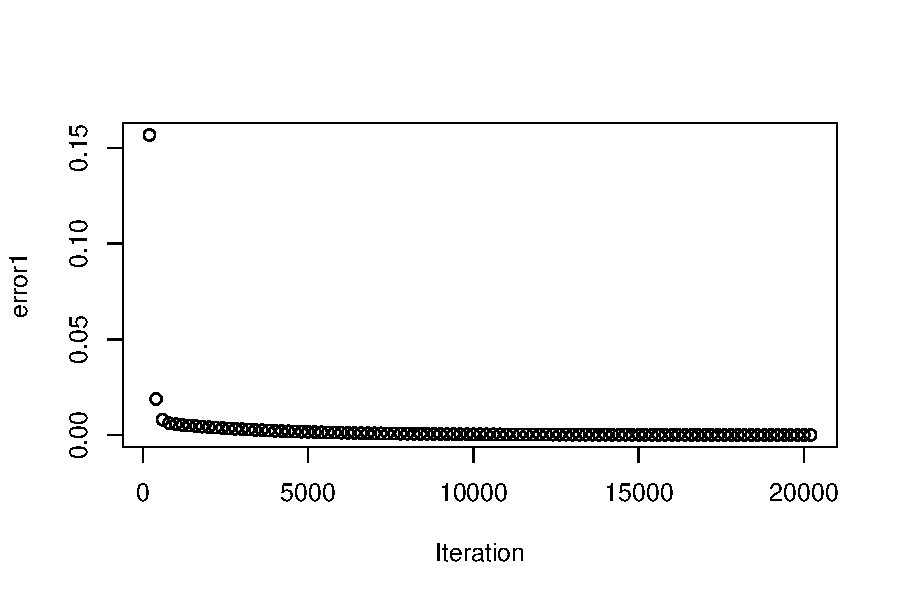
\includegraphics[width = 0.4\textwidth]{Graphs/Error1.pdf}
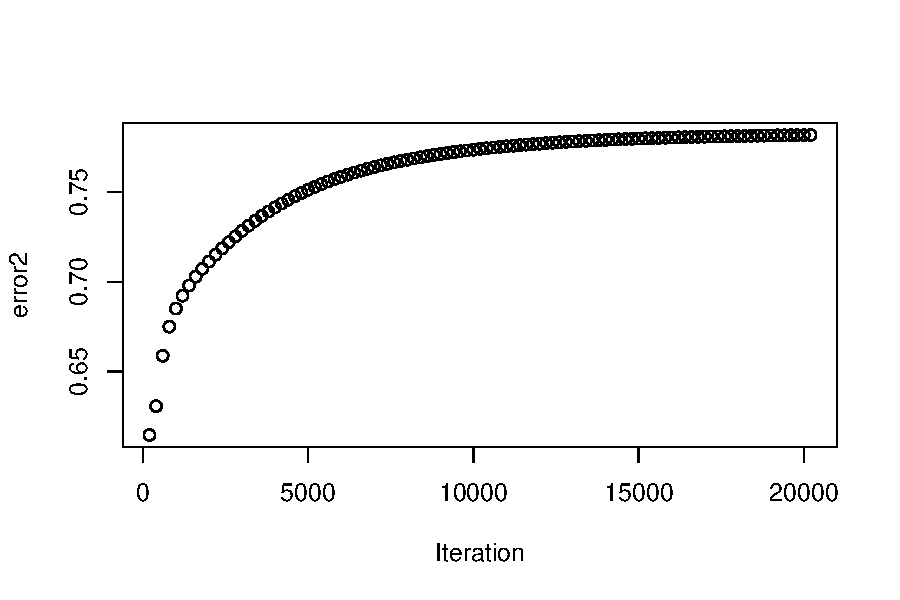
\includegraphics[width = 0.4\textwidth]{Graphs/Error2.pdf}
\end{figure}



\end{document}